\documentclass[preprint,3p,onecolumn,times,review]{elsarticle}
%\documentclass[preprint,3p,twocolumn,times]{elsarticle}
%\documentclass[preprint]{elsarticle}
%\usepackage[square, sort, numbers]{natbib}
\usepackage[cmex10]{amsmath}
\usepackage{graphicx}
\usepackage{bussproofs}
\usepackage{booktabs}
%\usepackage{epstopdf}
%\epstopdfsetup{update} % only regenerate pdf files when eps file is newer
%\usepackage{color}
%\usepackage{epsfig}
%\usepackage{ascmac}
%\usepackage{alltt}
%\usepackage{float}
%\usepackage{stmaryrd}
%\usepackage{treeprint}
%\usepackage{fancyvrb}
%\usepackage[toc]{glossaries}
%\usepackage{lplfitch}

% \setlength{\jot}{4pt} % 



\title{An analysis of structural interoperability in ISO 13606\\ based on typed lambda calculus}

\author[plan]{Akimichi Tatsukawa\corref{cor1}}
\ead{akimichi.tatsukawa@gmail.com}
\address[plan]{Department of Planning, Information and Management, The University of Tokyo Hospital, Tokyo, Japan.}

\author[disease]{Emiko Shinohara}
\address[disease]{Center for Disease Biology and Integrative Medicine, Graduate School of Medicine, The University of Tokyo, Tokyo, Japan.}
\author[plan]{Takeshi Imai}
\author[plan]{Yoshimasa Kawazoe}
\author[plan]{Kazuhiko Ohe}

\cortext[cor1]{Corresponding author. Address: Department of Planning, Information and Management, The University of Tokyo Hospital, 7-3-1 Hongo, Bunkyo-ku, Tokyo, Japan, Fax: +81 3 3813 7238\\
\qquad Email address: akimichi.tatsukawa@gmail.com}

\newtheorem{thm}{Theorem}
\newtheorem{lem}[thm]{Lemma}
\newdefinition{rmk}{Remark}
\newproof{pf}{Derivation}


\begin{document}

\begin{frontmatter}

\begin{abstract}
  ISO 13606 defines a standard specification for exchange and integration of electronic health record (EHR) data with the goal of the interoperability of EHR data across heterogeneous systems.
  In order to achieve this goal, the standard provides a dual-model architecture in which archetypes are extensible schemas of EHR data via their specialization and composition mechanism.
  However, the standard lacks formal semantics of archetypes, which makes it difficult to build EHR systems or archetype repositories in a consistent and longitudinal manner.
  The goal of the present study was to clarify the archetype semantics of ISO 13606 by means of a formal methodology called typed lambda calculus, which has been widely used to define and analyze the semantics of modern programming languages and database systems.
  We focus on the variance and immutability of the archetype, because these factors determine the expressive power of archetypes.
  We defined a type system that represents the fundamental components of ISO 13606 semantics and analyzed the semantics based on a deductive system of the type theory.
  Our results indicate that the archetypes should be covariant and immutable schemas in order to guarantee both the interoperability of EHR data and the extensibility of archetypes.
\end{abstract}



\begin{keyword}
  ISO 13606 \sep Archetypes \sep Typed Lambda Calculus \sep Formal Semantics \sep openEHR
\end{keyword}

\end{frontmatter}

%\tableofcontents

\section{Introduction}

\subsection{Background}

The efficient use of medical resources and the fulfillment of large-scale clinical research requires integration of electronic healthcare record (EHR) systems that store diverse clinical data for long periods of time.
This challenge, however, remains.
Heterogeneity between various local EHR systems is a major reason why interoperabilities such as the construction of a central repository or an exchange of EHR data are not possible.
In order to achieve interoperability of EHR data from local systems in a consistent and longitudinal manner, the schema of EHR data must satisfy the requirements of various organizations and evolve over time in accordance with the development of medical concepts.

ISO 13606 defines a common healthcare model as an international standard.
The overall goal of the standard is "to devise a generalized approach representing every conceivable kind of health record data structure in a consistent way"\cite[vi]{iso08:13606_healt_elect_part1} so as to "support the interoperability of systems and components that need to communicate EHR data"\cite[v]{iso08:13606_healt_elect_part1}.
Due to the complexity and continuing evolution of the healthcare domain, the common model must meet the needs of organizations and cope with the progress of medical concepts.
In order to overcome these difficulties, ISO 13606 has adopted a dual-model approach that is based on the separation of concepts in two levels: (1) information and (2) knowledge.
Knowledge is represented by an archetype, which is formal model of a clinical concept\cite[p.158]{jesualdo06:_ontol_infras_seman_integ_clinic_archet}.

While this dual-model architecture is a major feature of ISO 13606, the  original idea stems from the openEHR specification, which was also an attempt at the "sharing of EHRs via interoperability at data and knowledge levels."\cite[p.12]{beale08:_openeh_archit_overv}

In fact, ISO 13606 is largely considered to be a subset of the full openEHR specification\cite{peter:_relationship_cen13606_hl7_openehr,chen09:_archet_conversion_ehr_model}. Therefore, both specifications share common features.
The present paper refers primarily to ISO 13606 as a standard for the interoperability of EHR systems. However, for the case in which the openEHR specification is more appropriate, we will refer to this specification.

\subsection{Objective}

As specifications become larger and more complicated, the consistency and correctness of the specifications become uncertain, and ISO 13606 is no exception.
The ISO 13606 specification describes the behavior of archetypes but does not define any formal semantics.
This is problematic because the lack of a definition makes implement an EHR system based on ISO 13606 difficult.
For example, when we define an archetype using both specialization and composition, are we allowed to combine them in an arbitrary manner? Or, are there constraints embedded in the semantics of the archetypes?

Since ISO 13606 does not provide a sufficient explanation regarding these questions, we must look back at the original openEHR specifications for clues.
In the two specifications, we found two important statements. One is cited from the ISO 13606 specification, and the other from the openEHR specification.

\begin{enumerate}[Assertion 1.]
\item[{\bf Assertion 1}]

  Any data created via the use of a specialized archetype shall be conformant both to it and to its parent\cite[viii]{iso08:13606_healt_elect_part2}.
\item[{\bf Assertion 2}]

  Data created with any specialized archetype will always be matched by queries based on the parent archetype\cite[p.51]{beale08:_openeh_archit_overv}.
\end{enumerate}

These assertions are prerequisites for laying the groundwork on archetype semantics, because they suggest the requirements for EHR data conformance and queries based on archetype.
However, the exact meanings remain unclear because natural language descriptions leave room for a wide range of interpretations.
For example, what does the phrase 'conformant to' mean exactly? How can we assure that certain queries match appropriate EHR data and that others do not?


The goal of the present study is to clarify the ISO 13606 archetype semantics by means of a formal methodology in order to support the above assertions. We will investigate the semantics in a formal manner under the assumption that at least these two assertions must hold and will pursue further consequences that are logically derived from the semantics.
The term 'formal methodology' refers to the situation in which every term in a syntax or every property in semantics is defined by a symbol so that each has a precise meaning that serves as a foundation for reasoning or verification. 

As a means of such formalization, we used {\bf typed lambda calculus}, which is a theory that is widely used as meta-language in the field of computer science to define and analyze the semantics of various programming languages and database systems \cite{ohori89:_simpl_seman_ml_polym,igarashi01:_feath_java}.
We believe that this formalization technique can contribute to the analysis of ISO 13606 in the same manner as previous domains in computer science.
To the best of our knowledge, this is the first attempt to apply typed lambda calculus to semantics in the medical field.

\section{Material and Methods}


\subsection{Concepts for EHR data integration\label{sec:higher_concepts}}

Before introducing the formal methodology of typed lambda calculus, we begin by explaining several concepts that are fundamental to the exchange and integration of EHR data.
These concepts are important because obtaining a final decision from different results based on a formal reasoning requires conceptual criteria that are higher than formalization itself.
In other words, formalization is the necessary requirement for building a solid semantics, but it is not sufficient.
When we encounter different results from different premises, we have to choose either one of the results even though these results are both valid in terms of formalization.
In order to achieve EHR data integration, these criteria are 'structural interoperability' and 'schema extensibility'.


\subsubsection{Structural interoperability should be guaranteed}


Every standardization of clinical information, including ISO 13606, attempts to achieve a certain level of interoperability between EHR systems.
However, definitions of interoperability in the standardizations vary between the standardizations.
ISO 13606 defines 'interoperability' as the "ability for data shared by systems to be understood at the level of fully defined domain concepts"\cite[p.5]{iso08:13606_healt_elect_part1}.
However, the term 'to be understood' is not precise in terms of computer science. Computers can never 'understand' the meaning of data, they only perform computations.
Moreover, we believe that the root of this ambiguity is due to the fact that two different types of concepts are being explained using one terminology.
Thus, we divided the concept of interoperability into two levels, as follows.

\begin{itemize}
\item Structural Interoperability
  
  Structural interoperability is defined as the ability to process data based on a shared formal schema and the sound semantics of the data. 
  This type of interoperability is referred to as 'structural' because modern database schemas or data models are solely concerned with the structure of data, such as field names, data types, and relations.
\item Semantic Interoperability

Semantic interoperability is defined as the ability to process data based on the shared meanings of terms, as similarly stated in \cite{veltman01:_syntac_seman_inter,sebastian09:_towar_seman_inter_for_elect_healt_recor,maldonado07:_framew_for_clinic_data_stand_based_archet,martinez-costa10:_iso_en_openeh,jose09:_linkeh_ed}.
  The meanings of terms can be shared by annotating data items with extra labels, which are not exactly structure.
  This type of interoperability is referred to as 'semantic' because we can distinguish two data by looking at their annotated labels, even if the data are structurally identical.
\end{itemize}

Comparing these two aspects of interoperability, structural interoperability is more fundamental than semantic interoperability for EHR data integration, because semantic annotations are useful only if the annotated attribute represents a valid value.
In investigating the archetype semantic, we concentrate  on the concept of structural interoperability.

\subsubsection{EHR schema should be extensible}

When we build every EHR system based on a unified and fixed EHR schema, we can easily achieve structural interoperability.
In real settings, however, building a single giant schema is difficult especially in the medical domain, where concepts are not only large but also open-ended with breadth, depth, and complexity, because new information, finer-grained detail, and new relationships are always being discovered in medicine \cite{rector99:_clinic_termin,renner96:_data_inter}.

The following example, which is a longitudinal cancer cohort study, illustrates the difficulties involved (Fig. \ref{fig:cohort_study}).
At the starting of the study, we store smoking histories as the exposure level and several tumor markers as surrogates for cancer outcome.
When a novel marker is discovered during the course of the study, we want to add the marker as an additional item, such as {\sf RevisedOutcome} in {\sf RevisedCase} (Fig. \ref{fig:cohort_study}).
Or, if an unexpected exposure, such as a nuclear plant accident, is observed, the extra exposure (in this case, a dose of irradiation) should be added.

As this example indicates, when data are stored and traced longitudinally, the EHR schema must be extended as medicine progresses. Otherwise, a number of disorganized schemas, many of which are similar but slightly different, will accumulate, and the cost of maintenance will increase significantly.


\begin{figure}[!htbp]
  \begin{center}
    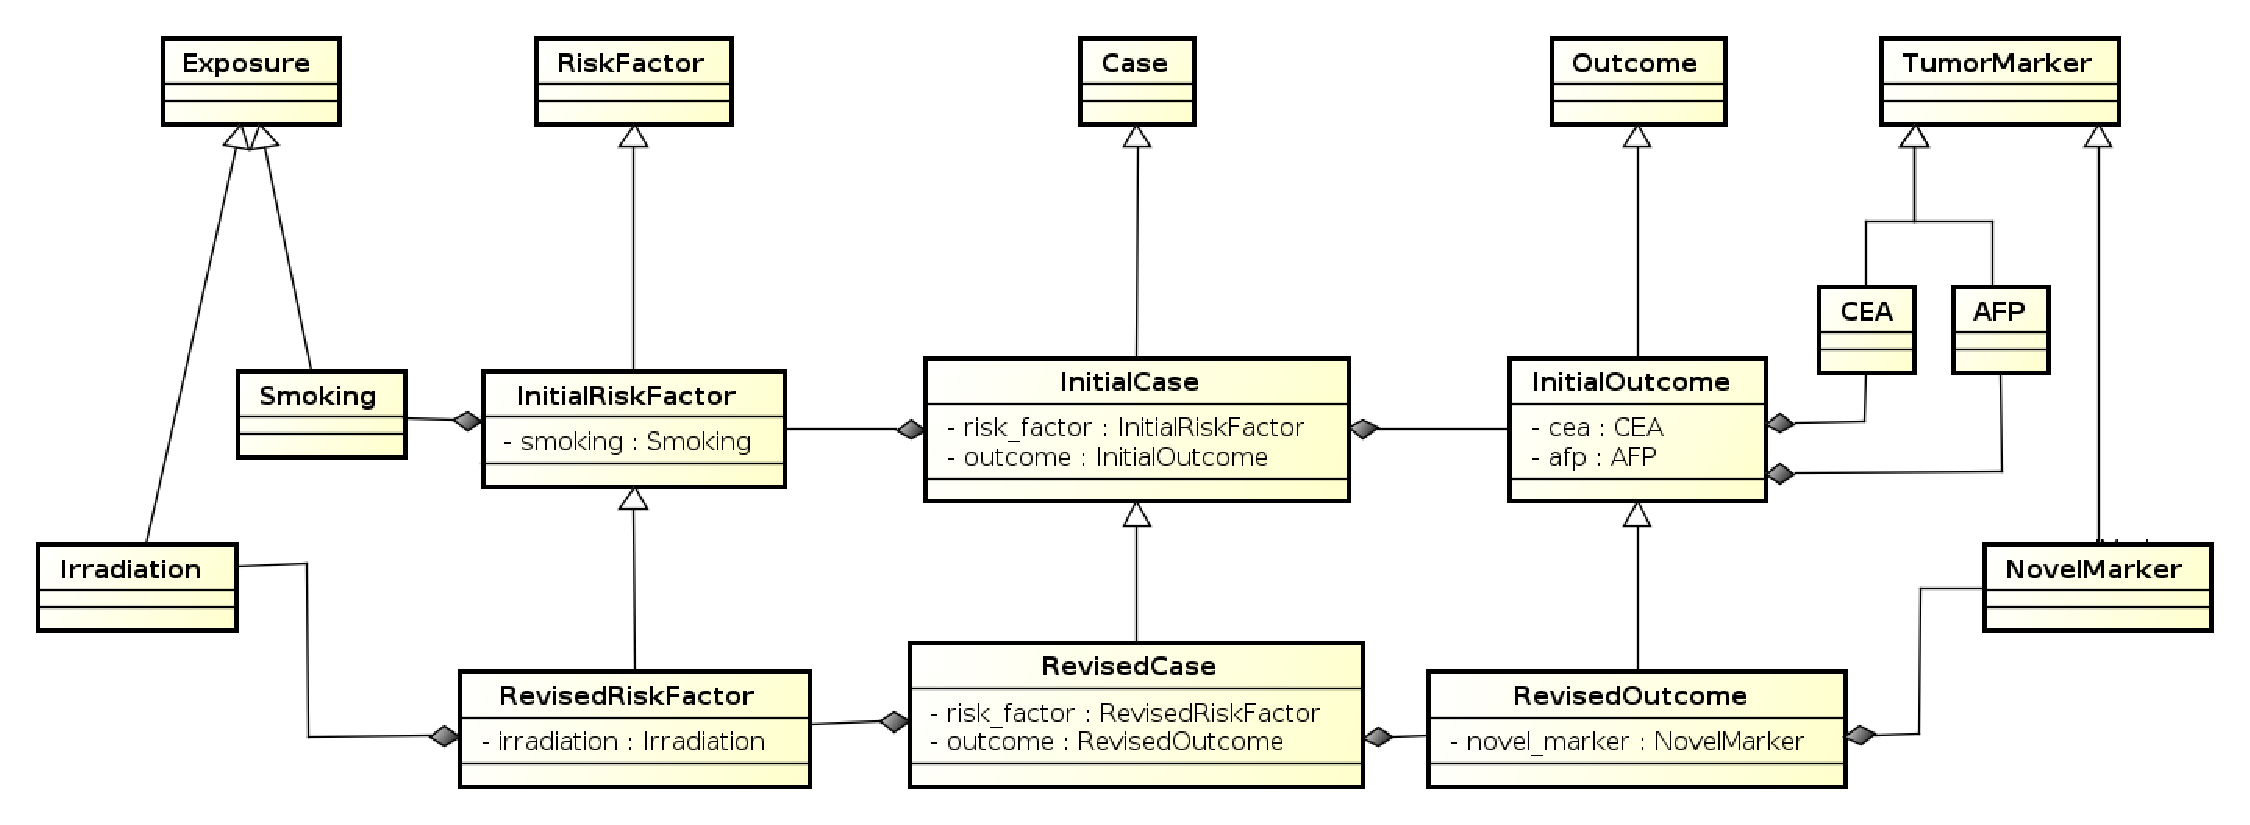
\includegraphics[width=14cm]{cancer_cohort_study_schema.eps}  
  \end{center}
  \caption{Unified modeling language diagram of an imaginary cohort study}\label{fig:cohort_study}
  The diagram describes the schema of an imaginary cohort study in chronological order.
  The lower diagram indicates the more recent content.
\end{figure}

\subsection{ISO 13606 architecture}

In this section, we present an overview of ISO 13606 for modeling architecture.
In particular, we focus on dual-model architecture and the specialization and composition of archetypes.
At the end of this section, we point out the problem associate with their combination (variances).

\subsubsection{Dual-model approach}


ISO 13606, like openEHR, adopts a dual-model architecture (Fig. \ref{fig:dual_model_approach}) to guarantee interoperability and support flexibility of the EHR schema.
The architecture has a Reference Model (RM) and an Archetype Model (AM) in the lower layer and archetypes in the upper layer.
The primary feature of the modeling architecture is to construct archetypes from the components of the RM and the AM.

\begin{figure}[!htbp]
  \begin{center}
    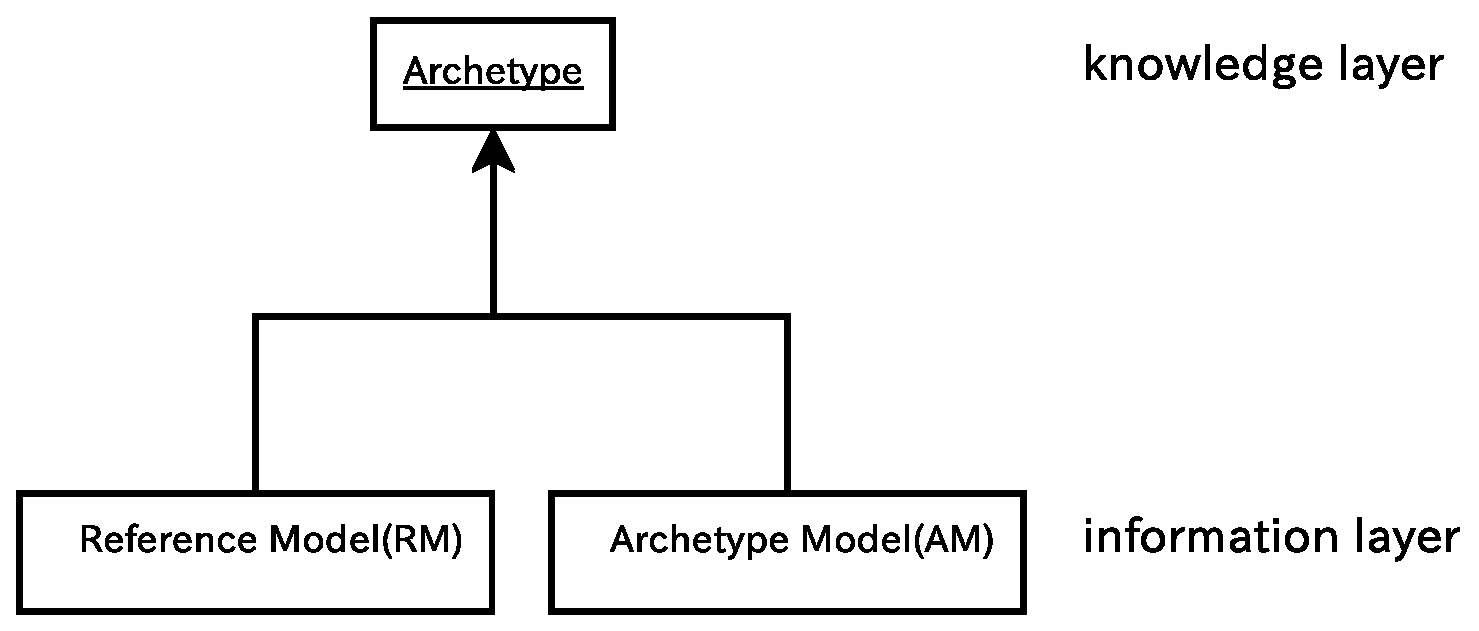
\includegraphics[width=7cm,clip]{dual_model_approach.eps}  
  \end{center}
  \caption{Dual-model approach}\label{fig:dual_model_approach}
  The diagram describes the dual-model architecture of ISO 13606, which consists of two layers, an information layer and a knowledge layer. The left-hand side of the figure indicates the information layer, in which the Reference Model and the Archetype Model are located, and the right-hand side indicates the knowledge layer, in which the Archetype resides.
  The arrows between these two layers indicate the dependency between the two layers, i.e., the combination of the RM and the AM yields an Archetype.
\end{figure}


The lower layer of the dual-model architecture contains a Reference Model and an Archetype Model.
The {\bf Reference Model} defines a set of data types and data structure from which any health record information is composed \cite[p.vi]{iso08:13606_healt_elect_part1}.
The model sits in the lower layer of the dual-model architecture, and represents the generic properties of health record information. \cite[p.vi]{iso08:13606_healt_elect_part1}.
In short, the model forms the generic building blocks of the EHR and contributes to interoperability, data consistency, and data quality.

The {\bf Archetype Model} is another component in the lower layer, and the model acts as a skeleton or template for archetypes.
The AM is an "information model of the metadata to represent the domain-specific characteristics of electronic health record entries"  \cite[p.2]{iso08:13606_healt_elect_part1}.
The model consists of "identifying information, a description (its metadata), a definition (expressed in terms of constraints on instances of an object model), and an ontology" \cite[p.vii]{iso08:13606_healt_elect_part2}.
The definition section includes a specification of the hierarchical schema to which instances of data (i.e., EHR data) shall conform.
The section defines the hierarchical organization of a set of nodes and constraints on the permitted values of attributes and data values \cite[p.6]{iso08:13606_healt_elect_part2}.
In other words, the AM defines the structure and constraints of EHR data from the combinations of the RM entities in their definition section.
On the other hand, the ontology section defines all linguistic entities in the archetype.
The section provides "the textual description for each concept from the definition section and bindings to other terminologies" \cite[p.871]{costa11:_clinic}, so that "the archetypes can be natural-language- and terminology-neutral" \cite[vii]{iso08:13606_healt_elect_part2}.

Looking back at the definitions of interoperability, we found that the definition and ontology sections in the AM correspond to each level of interoperability.
The definition section defines the structure and constraints of the EHR data, and so is a means of assuring structural interoperability.
In contrast, the ontology section binds an attribute with meaningful terminology, and so is a means of assuring semantic interoperability \cite[p.586]{duftschmid10:_extrac_elect_healt_recor_entit}.

The {\bf Archetype} resides in the upper layer of the dual-model architecture.
Archetypes define clinical concepts in the form of structured and constrained combinations of the entities of an RM.
While the difference between an Archetype and the AM is confusing, they reside on different layers, as shown in Fig. \ref{fig:dual_model_approach}.
The AM is static because it is defined by the specification in advance, whereas Archetypes are dynamic because they can be constructed at any time.
At this stage, the significance of the dual-model architecture is revealed.
In ordinary architectures that have only one layer of modeling, data models or a schema is already defined in a system or specification, which makes it difficult or impossible to modify or extend the schema.
In contrast, dual-model architectures statically include the basic components of schemas and the general mechanism for their construction, and the actual schemas are constructed dynamically from these components.


\subsubsection{Specialization and composition of archetypes}

The dual-model architecture enables the EHR schema to be defined dynamically and thus realizes Archetype flexibility.
Moreover, ISO 13606 provides a method by which to further enhance flexibility, namely, specialization and composition of archetypes.
With this mechanism, we can gradually extend the EHR schema in accordance with the progress of medicine or research.

First, archetypes may be specialized. New archetypes can be defined by further constraining the parent archetype.
Similar to class inheritance in object-oriented languages, the child of an archetype inherits all its attributes from the parent archetype and adds new items or refines existing items in the child archetype.

Second, archetypes may be composed \cite[ix]{iso08:13606_healt_elect_part2}. New archetype can be defined by containing other archetypes when they are specified in 'slots' of the new archetype (Fig. \ref{archetype_slot_regex}).
Similar to class composition in object-oriented languages, this 'composition' mechanism allows large data structures to be flexibly constrained via the hierarchical re-use of smaller archetypes. \cite{beale08:_openeh_archit_overv,beale07:_archet_objec_model}
Note that the specification allows a composed archetype to be specified either by stating a unique archetype identifier, or vaguely by wildcards (i.e., matches many possible archetypes) \cite[p.61]{beale07:_archet_defin_languag}. This issue is discussed later herein.

\begin{figure}[!htbp]
\begin{verbatim}
SECTION  [at2000] occurrences matches {0..1} matches {
  items matches {
     allow_archetype SECTION occurrences matches {0..*} matches {
        include
           id matches {/.*\.iso-ehr\.section\..*\..*/}
        exclude
           id matches {/.*\.iso-ehr\.section\.patient_details\..*/}
     }
   }
}
\end{verbatim}
  \caption{Excerpt of architecture description language with archetype \_slot}\label{archetype_slot_regex}
  This fragment of architecture description language defines an archetype slot, indicating which SECTION archetypes are allowed and excluded under the items property.
  Note that regular expressions are used to designate the allowed and excluded archetypes.
\end{figure}


\subsubsection{Variances of archetype \label{sec:variances_archetype}}

When we define an archetype by combining specialization and composition, we encounter several possibilities, referred to as variances. The variance of a type is said to be covariant in its components when the type varies in the same direction as one of its parts with respect to subtyping. The variance of a type is said to be contravariant when the type varies in the opposite direction as one of its parts with respect to subtyping. Finally, the variance of a type is said to be invariant if the type is neither covariant nor contravariant (Fig. \ref{fig:archetype_variances}).


\begin{figure}[!htbp]
  \begin{center}
    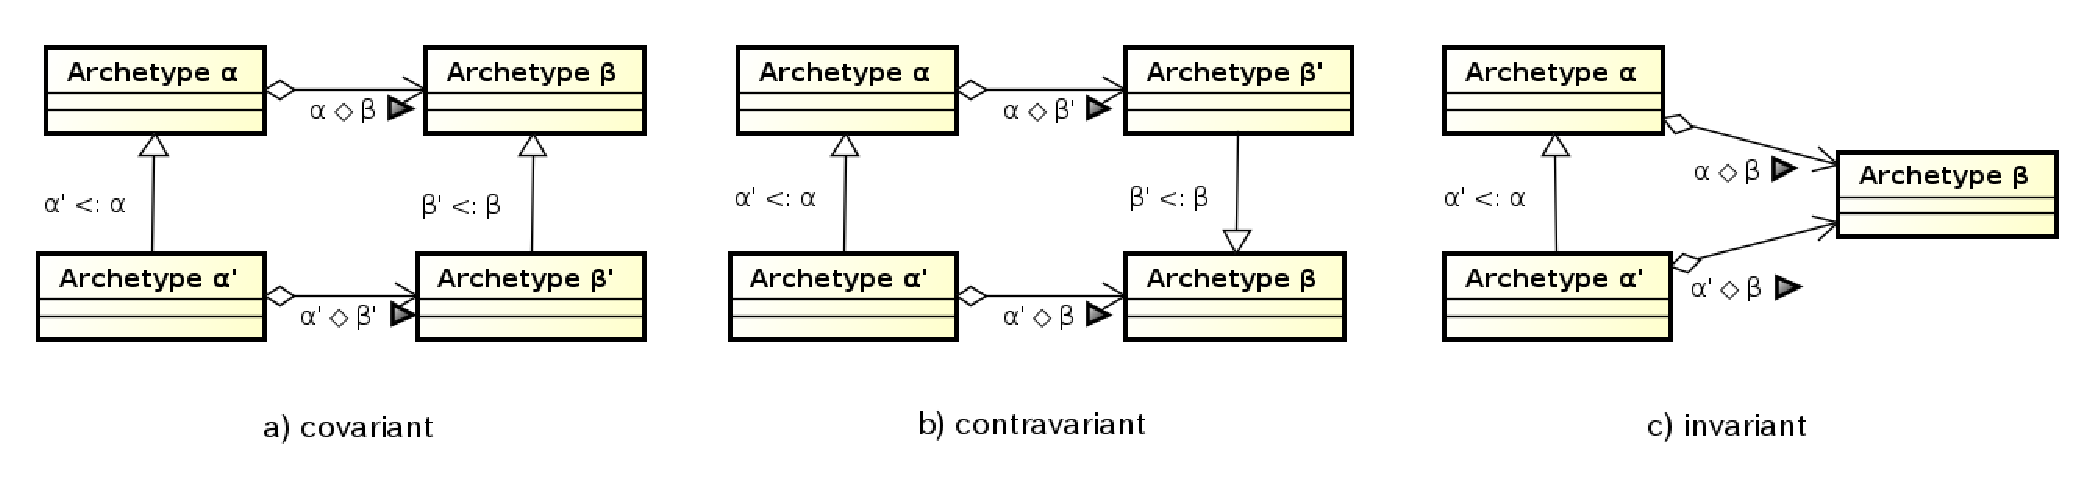
\includegraphics[width=16cm]{archetype_variance.eps}  
  \end{center}
  \caption{Three alternatives of archetype variances}\label{fig:archetype_variances}
  The figure shows three alternative archetype variances. a) Covariant: if $\alpha' <: \alpha$ and $\beta' <: \beta$, then $\alpha' \diamond \beta' <: \alpha \diamond \beta$, b) contravariant: if $\alpha' <: \alpha$ and $\beta' <: \beta$, then $\alpha' \diamond \beta <: \alpha \diamond \beta'$, and c) invariant: if $\alpha' <: \alpha$ and $\beta'= \beta$, then $\alpha' \diamond \beta <: \alpha \diamond \beta$.
  Note that, in this figure, the operator $<:$ denotes 'subtype of', and $\diamond$ means 'composed of'.
\end{figure}

The actual variance of an archetype depends on the semantics of the archetype, i.e., how the archetype is constructed as a type. We consider this problem to be a major issue in archetype semantics because it affects the archetype expressiveness and extensibility as EHR schemas.


\subsection{Typed lambda calculus}

In this section, we briefly introduce typed lambda calculus, which is our tool to investigate the archetype semantics. Lambda calculi are mathematical abstractions of computations, and in the typed lambda calculus, every variable must be explicitly typed. 
We herein use the terms typed lambda calculus and type theory interchangeably.

\subsubsection{How type theory is applied to ISO 13606}

Before introducing the details of typed lambda calculus, we present an overview of the correspondence between components of typed lambda calculus and ISO 13606.
In an abstract sense, types are containers that hold values, and so every model in ISO 13606 can be encoded as a type.
However, we must carefully decide which types can be assigned to each component of ISO 13606, because each type has its own characteristics.

We encoded the RM components without any internal structure as primitive types in type theory.
Not surprisingly, a string in the RM is mapped to the string type, and structured components are mapped to structured types in type theory, such as record type, variant type, and list type.
For example, the TEXT type in ISO 13606 has charset, languages, and originalText as its field \cite[p.36]{iso08:13606_healt_elect_part1}.
Therefore, the TEXT type can be encoded as a record type using Eq.~\ref{eqn:text_as_record}.
Note that in the present paper, concrete types, such as {\sf Record} or {\sf CS}, start with a capital letter and are shown in {\sf SansSerif} font.


\begin{alignat}{3}
  \mathsf{TEXT} \equiv \mathsf{Record}\{charset : \mathsf{CS}, languages : \mathsf{CS}, originalText : \mathsf{String} \}  \label{eqn:text_as_record}
\end{alignat}

Archetypes, which also have some internal structures, are encoded in record types.
For example, the vital signs archetype (Fig. \ref{fig:vital_signs_archetype}) can be encoded as shown in Eq.~\ref{eqn:vital_signs_record}.
The specialization of archetypes corresponds to Record subtyping, and the composition of archetypes corresponds to Record nesting.

\begin{figure}[!htbp]
\begin{verbatim}
definition
   SECTION[at0000] matches {   -- Vital signs
      items cardinality matches {2} matches {
         allow_archetype OBSERVATION[at0001] matches {
            include
               archetype_id/value matches {"openEHR-EHR-OBSERVATION.blood_pressure.v1"}
         }
         allow_archetype OBSERVATION[at0002] matches {
            include
               archetype_id/value matches {"openEHR-EHR-OBSERVATION.body_temperature.v1"}
         }
      }
   }
\end{verbatim}
  \caption{Excerpt of the vital signs archetype} \label{fig:vital_signs_archetype}
  This is an example of a definition section in the vital signs archetype.
  Note that we modified the certified archetype in the Clinical Knowledge Manager (CKM) repository to match the explanation herein.
\end{figure}


\begin{alignat}{3}
  \mathsf{VitalSigns} \equiv \mathsf{Record}\{definition[at0000] : \mathsf{Record}\{&items[at0001] : \mathsf{BloodPressure},\nonumber\\
                                                                              &items[at0002] : \mathsf{BloodTemperature;}\}\} \label{eqn:vital_signs_record}
\end{alignat}

EHR data are instances of Archetypes, \footnote{Note that this is not an "archetype instance", which is defined as a metadata class instance of an archetype model in the ISO 13606 specification \cite[p.2]{iso08:13606_healt_elect_part1}.} i.e., instances of the corresponding Record type, because each EHR datum is created according to the corresponding archetype.
For example, Eq.~\ref{eqn:vital_signs_instance} yields an EHR datum for the vital sign archetype of Eq.~\ref{eqn:vital_signs_record}.
Note that instance names are written in lower case, e.g., $record$, and the details of $\mathsf{BloodPressure}$ and $\mathsf{BloodTemperature}$ are omitted for clarity in this equation.


\begin{alignat}{3}
  vital\_signs \equiv record\{definition[at0000] : record\{&items[at0001] : record\{systolic: 120, diastolic : 80\},\nonumber\\
                                                                    &items[at0002] : record\{temperature: 37.5, unit : C\}\}\} \label{eqn:vital_signs_instance}
\end{alignat}


Table \ref{tab:correspondence} summarizes our assignment of ISO 13606 to type theory.
We believe that these assignments are intuitively plausible, as explained above.
However, this does not exclude other possibilities of assignments, which might lead to different results from those of the present study.

\begin{table}[!htbp]
  \centering
  \caption{Correspondence between type theory and ISO 13606}\label{tab:correspondence}
  \begin{tabular}{ccc}
    \toprule%[1.5pt]
    ISO 13606 & type theory \\
    \midrule
    primitive types in RM & basic types \\
    data structures in RM & structured types \\
    archetype & record type \\
    EHR data & instances of record type\\
    \bottomrule%[1.5pt]
  \end{tabular}
\end{table}


\subsubsection{Introducing types}

We presented the minimum set of typed lambda calculus as long as it was sufficient to provide the basis for our purpose, the purpose to clarify archetype semantics by means of formalization in support of the aforementioned two assertions.
We start from fundamental types, such as the function type or basic types, and progressively extend the system with more complex types, such as record or variant type (Table \ref{tab:types_notations}).
For a more comprehensive explanation of type theory, see for instance,\cite{pierce02:_types_progr_languag,mitchell00:_found_progr_languag,harper13:_pract_found_progr_languag}.


\begin{table}[!htbp]
  \centering
  \caption{List of major types and corresponding notation used in the present study}\label{tab:types_notations}
  \vspace{6pt}
  \begin{tabular}{lcrr}
    \toprule %[1.5pt]
    type &  & notation \\
    \midrule
    function type &  & \(\tau \rightarrow \sigma \)\\
    basic type    &  & \(\mathsf{String}, \mathsf{Boolean}\), etc.\\
    structured type &  \\
    & record & \(\mathsf{Record}\)\\
    & variant & \(\mathsf{Variant}\)\\
    & list & \([\tau]\)\\
    \bottomrule%[1.5pt]
  \end{tabular}
\end{table}

First, a formal assertion relating entities such as terms or types under a certain environment, is referred to as a {\bf judgment} (Eq.~\ref{eqn:judgment}).
The expression $\Gamma ~ \vdash M:\tau$ should be read as "a term M has a type of $\tau$ under an environment $\Gamma$". We write $\Gamma ~ \vdash \tau$ to express that $\tau$ is a well-formed type under the environment $\Gamma$. In either case, $\Gamma$  is a set of assumptions about the types of free variables in $M$ and is referred to as the {\bf type environment}.

\begin{alignat}{3}
  & {\Gamma~ \vdash \Omega} \qquad  \text{(judgment)}  \label{eqn:judgment}
\end{alignat}


In typed lambda calculus, every term has a type that is a collection of values with shared characteristics.
The types are introduced into the system by adding {\bf typing rules}, such as those given by Eq.~\ref{eqn:function_type_rule}.
These typing rules assert the validity of certain judgments based on other judgments that are known to be  valid.
The judgments above the horizontal line are referred to as the premises of the rule, and those below the horizontal line are referred to as the conclusion.

The most fundamental type is the Function Type ($\tau \rightarrow \sigma$), which satisfies the typing rule given by Eq.~\ref{eqn:function_type_rule}.
The notation $(M~N)$ denotes a function application in which a function $M$ is applied to the argument $N$.
When we apply the term $M$ of function type $\tau \rightarrow \sigma$ to the value of type $\tau$, we obtain the term of type $\sigma$ (Eq.~\ref{eqn:application}).
This function type appears in database queries (such as Eq.~\ref{eqn:query_by_foldr}), because a query is a function that accepts a database and returns a result set of the database.


  \begin{align}
        \text{Typing rules:} \qquad   \nonumber\\
    & \frac{\Gamma~ \vdash \tau \qquad \Gamma~ \vdash \sigma}
           {\Gamma~ \vdash \tau \rightarrow \sigma}  & \label{eqn:function_type_rule} \text{(function type)}\\[6pt]
    & \frac{\Gamma \vdash M:\tau \rightarrow \sigma \qquad  \Gamma \vdash N:\tau}
           {\Gamma ~ \vdash (M~N):\sigma} & \qquad \text{(application)} \label{eqn:application}
  \end{align}


Because EHR data are aggregates of various types of data, we need to introduce such data types.
For example, blood pressure data are constructed as aggregates with the numeric type for the pressure value and a string type for the unit of measurement.

We classify these data types into two categories: basic and structured.
Basic types, such as Boolean or Integer,  are primitive data types in that they lack any internal structure.
When these primitive types are built in BasicType, they are available in our system as Eq.~\ref{eqn:basic_type_rule}.
$\Gamma~ \vdash \diamond$ means that $\Gamma$ is well-typed, which means that the type environment $\Gamma$ has nothing but valid types.
  
\begin{figure}[!htbp]
  \begin{align}
    \frac{\Gamma~ \vdash \diamond \qquad \tau \in \mathsf{BasicType}}
    {\Gamma~ \vdash \tau} \label{eqn:basic_type_rule}
  \end{align}
\end{figure}

EHR data are inherently structured in that they consist of large collections of data entities of several types.
Thus, we introduce such structured data types into our type system in order to capture the ISO 13660 data model. Note that, in the present study, we use M and N as terms $\tau$ and $\sigma$ for meta-variables over type.
  
\begin{itemize}
\item Record Types

  A record type is a cross-product of the values with a projection operation for extracting components by name \cite[p.18]{cardelli04:_type_system,pierce02:_types_progr_languag}.

  The definition of structured type has three sections. In the record type, the terms section defines syntactic forms of a record and its projection (Eqs.~\ref{eqn:record_construction} and \ref{eqn:record_projection}). The types section defines the $\mathsf{Record}$ type (Eq.~\ref{eqn:record_type}). The typing rules section defines rules for the type of record construction and its projection (Eqs.~\ref{eqn:record_constructiontyping_rule} and \ref{eqn:record_projection_typing_rule}). Note that $i \in 1..n$ is shorthand for $\{ i~|~ i  \in \mathbb{N} \wedge 1 \leq i \wedge i \leq n )\}$, which indicates that the variable $i$ ranges over natural numbers from 1 to $n$.

    \begin{alignat}{4}
        \text{Terms:} \qquad   \nonumber\\
        M~ & {::= \dots }\nonumber\\
           & | ~~ record\{l_1 = M,\dots,l_n = M \} & (\text{record construction}) \label{eqn:record_construction}\\
           & | ~~M.l_i    & (\text{record projection}) \label{eqn:record_projection}\\
        \text{Types:} \qquad   \nonumber\\
        \tau~  & {::= \dots}\nonumber\\
               &  |~~ \mathsf{Record}\{l_1 : \tau, \dots l_n : \tau \} \label{eqn:record_type}\\
        \text{Typing rules:} \qquad   \nonumber\\
        & \frac{\Gamma \vdash M_i:\tau_i}
               {\Gamma ~ \vdash record\{l_i: M_i\}: \mathsf{Record}\{l_i : \tau_i\}} \qquad where~i \in 1..n \label{eqn:record_constructiontyping_rule} \\[6pt]
        & \frac{\Gamma \vdash M : \mathsf{Record}\{l_i : \tau_i\}}
               {\Gamma ~ \vdash M.l_i : \tau_i} \qquad where~i \in 1..n \label{eqn:record_projection_typing_rule}
     \end{alignat}
   
\item Variant Type
  
  While the record type requires all of the fields to be set by values, there is a case in which only one of the fields must be filled in.
  Figure \ref{fig:example_variant_type} is an example of such a case, and this fragment of the archetype should be encoded as a variant type.
  The variant type, which is a named disjoint union of types, is a type into which values fall into a limited number of categories \cite{pierce02:_types_progr_languag,cardelli04:_type_system}.

  \begin{figure}[!htbp]
    \begin{verbatim}
            DV_CODED_TEXT matches {
              defining_code matches {
                [local::
                 at1000, -- Hepatitis A
                 at1001 -- Hepatitis B
                ]
              }
            }
    \end{verbatim}
    \caption{Example of a Variant Type in DV\_CODED\_TEXT}\label{fig:example_variant_type}
    This fragment is an example of a variant type and defines a constraint of type DV\_CODED\_TEXT, the value of which should be either hepatitis A or B.
  \end{figure}

\item List Types

  EHR data often contain a series of events, such as a Holter electrocardiogram.
  The list type has finite-length sequences of the same type that describe a series of events and is widely used in numerous programming languages, as well as in ISO 13606 \cite{cardelli04:_type_system,pierce02:_types_progr_languag,geuvers09:_introd_type_theor}.
  In the present paper, $[\tau]$ describes finite-length sequences in which the element are taken from $\tau$.
\end{itemize}


\subsubsection{Subtyping}

EHR data may be organized hierarchically.
In Fig. \ref{fig:excerpt_reference_model}, for example, {\sf ELEMENT} and {\sf CLUSTER} are subordinate to {\sf ITEM} in their hierarchy, because each subordinate class (i.e., {\sf ELEMENT} and {\sf CLUSTER}) inherits all of the members of its parent class {\sf ITEM}.
This hierarchical relation, which is implemented as inheritance in object-oriented languages, is formalized as {\bf subtyping} in type theory\cite[p.85]{craig07:_objec_orien_progr_languag}.
In this section, we introduce general rules for subtyping and specific rules for each type.
When we define the specific subtyping rules so as to be compatible with the general rules, we are able to check the validity of a given subtyping based on a deductive system of the type theory.

\begin{figure}[!htbp]
  \begin{center}
    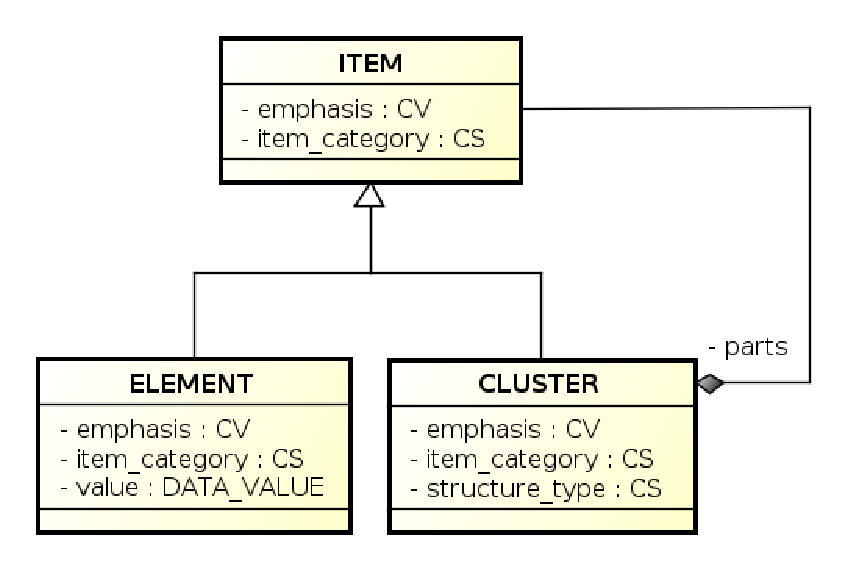
\includegraphics[width=6cm]{excerpt_reference_model.eps}  
  \end{center}
  \caption{Excerpt of the ISO 13606 Reference Model}\label{fig:excerpt_reference_model}
  This unified modeling language diagram is an excerpt from the ISO 13606 Reference Model\cite[p.10]{iso08:13606_healt_elect_part1} and defines the hierarchy of {\sf ITEM} and its subordinate {\sf ELEMENT} and {\sf CLUSTER}.
\end{figure}

The central theorem of subtyping is the {\bf subsumption principle} (Eq.~\ref{eqn:subsumption_rule}), which says that if type $\tau'$ is a subtype of $\tau$, then an instance of type $\tau'$ can be used in any context in which an instance of type $\tau$ can appear.
In subtyping, the operator '$<:$' is a reflexive transitive closure (Eqs.~\ref{eqn:subtyping_reflexive} and \ref{eqn:subtyping_transitive}) similar to the numeric comparison operator '$\leq$', so that  $\tau' <: \tau \text{ and}~ \tau <: \tau' $ means that $\tau \text{ is equal to } \tau'$ (cf., $a \leq b \text{ and}~ b \leq a $ means that $a = b$).

\begin{alignat}{2}
        \text{Typing rules:} \qquad   \nonumber\\
        & \frac{\Gamma~ \vdash M : \tau'  \qquad \Gamma~ \vdash \tau' <: \tau}
               {\Gamma~ \vdash M : \tau} & \text{(subsumption principle)}\label{eqn:subsumption_rule}\\[6pt]
        & \frac{\Gamma~ \vdash M : \tau}
               {\Gamma~ \vdash \tau <: \tau} & \label{eqn:subtyping_reflexive} \text{(reflexive)}\\[6pt]
        & \frac{\Gamma~ \vdash \tau'' <: \tau' \qquad \Gamma~ \vdash \tau' <: \tau}
               {\Gamma~ \vdash \tau'' <: \tau} & \label{eqn:subtyping_transitive} \text{(transitive)}
\end{alignat}


Subtyping rules should be defined for each type, and every subtyping rule should be compatible with the subsumption principle.
We presented the subtyping rules for structured types. In the record type, 
one record type is a breadth subtype of another if the first has at least all of the fields of the second (Eq.~\ref{eqn:record_width_subtyping}), and the other record type is a depth subtype of another if they have exactly the same fields, but the types of the corresponding fields are subtypes (Eq.~\ref{eqn:record_depth_subtyping}).
The depth subtyping rule for the variant type is identical to that of the record type (cf., Eqs.~\ref{eqn:variant_depth_subtyping} and \ref{eqn:record_depth_subtyping}), but the breadth subtyping rules for the variant type is different from that for the record type. A subtype of the variant type cannot have more fields than its supertype (Eq.~\ref{eqn:variant_width_subtyping}).

Since we abstracted archetypes as record types, archetype specialization can be modeled as record subtyping. We can add new items or modify the existing items in the specialized archetype as long as the extensions are compatible with Eqs.~\ref{eqn:record_width_subtyping} and \ref{eqn:record_depth_subtyping}.

\begin{figure}[!htbp]
  \begin{alignat}{3}
    \text{Record subtyping rules:} \qquad   \nonumber\\
    & \frac{\Gamma \vdash \tau_i \qquad where~i \in 1..n+m} 
           {\Gamma ~ \vdash \mathsf{Record}\{l_i : \tau_i\}_{i \in 1..n+m}  <: \mathsf{Record}\{l_i: \tau_i\}_{i \in 1..n}}  & \label{eqn:record_width_subtyping}\\[6pt]
    & \frac{\Gamma \vdash \tau'_i <: \tau_i}
           {\Gamma ~ \vdash \mathsf{Record}\{l_i: \tau'_i \}  <: \mathsf{Record}\{l_i: \tau_i\}}  \qquad where~i \in 1..n & \label{eqn:record_depth_subtyping}\\
    \text{Variant subtyping rules:} \qquad   \nonumber\\
    & \frac{\Gamma \vdash \tau_i \qquad where~i \in 1..n+m} 
           {\Gamma ~ \vdash \mathsf{Variant}\{l_i : \tau_i\}_{i \in 1..n}  <: \mathsf{Variant}\{l_i: \tau_i\}_{i \in 1..n+m}}  & \label{eqn:variant_width_subtyping}\\[6pt]
    & \frac{\Gamma \vdash \tau'_i <: \tau_i}
           {\Gamma ~ \vdash \mathsf{Variant}\{l_i: \tau'_i \}  <: \mathsf{Variant}\{l_i: \tau_i\}}  \qquad where~i \in 1..n & \label{eqn:variant_depth_subtyping}\\
    \text{List subtyping rule:} \qquad   \nonumber\\
    & \frac{\Gamma \vdash \tau' <: \tau}
           {\Gamma ~ \vdash [\tau'] <: [\tau]}                                                    & \label{eqn:list_subtyping_rule}
  \end{alignat}
\end{figure}

In addition, structured types, even basic types, can be subtyped by introducing an ad hoc subtyping rule \cite[p.28]{cardelli04:_type_system}.
When we define the ad hoc rules, their actual semantics should be compatible with the subtyping. Otherwise, the system is consistent in theory, but useless in reality.
For example, since we can regard an integer value as a real number (e.g., 1 as 1.0), a subtyping rule $\mathsf{Integer} <: \mathsf{Real}$ can be introduced.

This can also be applied to the structured types in the RM, as long as they are compatible with the ISO 13606 specification. According to Fig. \ref{fig:excerpt_reference_model}, for example, we can define subtyping between {\sf ELEMENT} and {\sf ITEM} as shown in Eq.~\ref{eqn:element_subtyping} and {\sf CLUSTER} and {\sf ITEM} as shown in Eq.~\ref{eqn:cluster_subtyping}.

\begin{alignat}{3}
  \frac{\Gamma~ \vdash \diamond}
       {\Gamma~ \vdash \mathsf{ELEMENT} <: \mathsf{ITEM}} \qquad \text{(ad-hoc)} \label{eqn:element_subtyping} \\[6pt]
  \frac{\Gamma~ \vdash \diamond}
       {\Gamma~ \vdash \mathsf{CLUSTER} <: \mathsf{ITEM}} \qquad \text{(ad-hoc)} \label{eqn:cluster_subtyping}
\end{alignat}



\subsubsection{Type system and its deductive system}

Deductive proofs are necessary in order to confirm the validity of the assertions under a given system.
When we define a number of type rules based on previous disciplines, the collection of axioms and typing rules is referred as a {\bf type system}.
In the given type system, we can construct a proof by combining the typing rules, and the proof is referred to as a {\bf derivation tree}.
Any derivation tree has leaves at the top and a root at the bottom, where each judgment is obtained from those immediately above it by applying some of the rules of the system.
Figure \ref{fig:example_derivation_tree} shows a simple example of a derivation tree. 
This deductive system is the most powerful feature of typed lambda calculus, because we can investigate the semantics of ISO 13606 with formal deductions. 


\begin{figure}[!htbp]
\begin{prooftree}
  \AxiomC{$\Gamma ~ \vdash \lambda x:\mathsf{Bool}.x:\mathsf{Bool} \rightarrow \mathsf{String}$}
  \AxiomC{$\Gamma ~ \vdash true:\mathsf{Bool}$}
  \RightLabel{[\ref{eqn:application}]}
  \BinaryInfC{$\Gamma ~ \vdash ((\lambda x:\mathsf{Bool}.x)~true) : \mathsf{String}$}
\end{prooftree}
\caption{Example of a derivation tree}\label{fig:example_derivation_tree}
This derivation tree indicates that the function of type $\mathsf{Bool} \rightarrow \mathsf{String}$ yields string type when applied to a boolean value. 
Note that the number in brackets to the right of the horizontal line indicates the equation number of the rule that was used (in this case, Eq.~\ref{eqn:application}). 
\end{figure}


\subsection{Application of type theory to ISO 13606}

In the previous sections, we introduced basic components of type theory and the correspondence of type theory to ISO 13606.
Next, we need to encode the problems in terms of this formal language in order to support the assertions (Assertions 1 and 2) and investigate the semantics of ISO 13606.

\subsubsection{How to formalize queries \label{sec:howto_formalize_queries}}

{\bf Assertion 2}, which states that ``data created with any specialized archetype will always be matched by queries based on the parent archetype'', is related to a requirement as to which queries and specialization should be obeyed.
Before deriving the assertion from the proposed type system, we encoded this assertion in terms of typed lambda calculus as follows.

Database theories \cite{hillebrand96:_datab_query_languag_embed_typed_lambd_calcul,grust99:_compr_queries,grust99:_how_compr_queries_funct,poulovassilis96:_algeb} tell us that the database can be presented as list of data, and its queries can be encoded as lambda terms and {\it foldr} (Eqs.~\ref{eqn:database_as_list} and \ref{eqn:query_by_foldr}).
Note that archetype is abbreviated as $\alpha$, N is a database containing a list of EHR data created by archetype $\alpha$, and $[~]$ is an empty list.
The database query has function type, because Eq.~\ref{eqn:query_by_foldr} indicates that $query~p$ takes a database that consists of a list of data (i.e., $[\alpha]$) and returns a result that also consists of a list of data (i.e., $[\alpha]$). The lambda term $p$ in Eq.~\ref{eqn:user_level_query} is a user-level query that is applied to each element of a collection, as $foldr$ calls itself recursively. The essential logic of query is embedded in term M. For instance, if we define $p \equiv \lambda x:\alpha.(\lambda xs:[\alpha].(\text{if}~ x.id == \text{"blood~pressure"} ~\text{then}~ x:xs ~\text{else}~ xs))$, then $query~p~N$ filters out the list of data for which the id field is "blood pressure".

\begin{alignat}{3}
   database \equiv & ~ N : [\alpha] \label{eqn:database_as_list}\\
   query~p  \equiv & ~ foldr~ p ~[~] : [\alpha] \rightarrow [\alpha] \label{eqn:query_by_foldr}\\
           & \text{where}  \quad   p \equiv \lambda~x:\alpha.(\lambda~xs:[\alpha].M) : \alpha \rightarrow [\alpha] \rightarrow [\alpha] \label{eqn:user_level_query} \quad \text{and,}\\
                  & \qquad   \text{{\it foldr} is a higher-order combinator for recursion \cite{hutton99:tutorial_universality_expressiveness_fold,bird92:_introd_funct_progr}} \nonumber
\end{alignat}


Based on these preconditions, {\bf Assertion 2} is formally expressed in Fig. \ref{fig:formalized_second_assertion}. The next task is to derive the judgment $(query~p)~N' :[\alpha] $ from these premises to support {\bf Assertion 2}.

\begin{figure}[!htbp]
\begin{alignat}{3}
  \text{provided that\quad}   & \Gamma \vdash \alpha' <: \alpha \text{, and}~ \\
                              & \Gamma \vdash query~p:[\alpha] \rightarrow [\alpha]\text{, and}~ \\
                              & \Gamma \vdash  N':[\alpha'] \\
  \text{then, derive\quad} & \Gamma \vdash (query~p)~N' :[\alpha] ~ & 
\end{alignat}\caption{Assertion 2 formalized}\label{fig:formalized_second_assertion}
Note that $\alpha$ is a parent archetype, $\alpha'$ is the specialized archetype of $\alpha$, and $N' : [\alpha']$ indicates ``a list of data created by the specialized archetype $\alpha'$''
\end{figure}


\subsubsection{How to introduce assignments for EHR data \label{sec:howto_introduce_assignments}}

Thus far, it has been impossible to update EHR data, because the record type that was introduced has only the projection operation and not the assignment operation for updating (Eq.~\ref{eqn:record_projection}).
Most of the programming languages and database systems, however, use destructive updating methods. In other words, old values are replaced by new values.
Therefore, we attempted to introduce update functionality to our system in order to determine what will happen to the archetype semantics.

In order to represent updatable EHR data, we introduced the additional types {\bf Reference type} and {\bf Unit type}. 
The Reference type is the mutable locations in memory \footnote{Interested readers can refer to Pierce \cite[p.159]{pierce02:_types_progr_languag} or Bruce \cite[p.77]{bruce02:_found_objec_orien_languag} for more concrete explanations.}, described as $\mathsf{Ref(\tau)}$ (Eq.~\ref{eqn:type_reference}). 
If term M has type $\mathsf{Ref(\tau)}$, then M denotes a location that can hold a value of type $\tau$. 
A datum can be updated by assignment operator ':=', the return type of which is Unit type (Eqs.~\ref{eqn:type_unit} and \ref{eqn:assignment}).


\begin{alignat}{3}
  \text{Types:} \qquad   \nonumber\\
                        \tau~ & {::= \dots }\\
                              & | ~~ \mathsf{Ref(\tau)}                           & \qquad \label{eqn:type_reference} \text{(type reference)}\\
                              & | ~~ \mathsf{Unit}                                & \qquad \label{eqn:type_unit} \text{(type unit)}\\
  \text{Typing rules:} \qquad   \nonumber\\
                              & \frac{\Gamma~ \vdash M:\mathsf{Ref(\tau)} \qquad \Gamma~ \vdash N:\tau}
                                      {\Gamma ~ \vdash M := N:\mathsf{Unit}} & \label{eqn:assignment} \qquad\qquad \text{(assignment)}
\end{alignat}

Thus, mutable EHR data were encoded as Archetype, the fields of which are $\mathsf{Ref}$ Type, i.e., $\mathsf{Archetype}\{l_i : \mathsf{Ref}(\tau_i)\}$. The typing rule of Archetype is given by Eq.~\ref{eqn:mutable_record_field_reference}, which indicates that the subtyping relation of mutable Archetype depends on the subtyping of Reference type. In the Results section of the present paper, we describe a critical change in the archetype semantics that is brought by this new encoding of the archetype.

\begin{alignat}{3}
  & \frac{\Gamma \vdash M_i : \mathsf{Ref}(\tau_i) }
         {\Gamma ~ \vdash archetype\{l_i: M_i\} : \mathsf{Archetype}\{l_i : \mathsf{Ref}(\tau_i) \} } \qquad  ~~(i \in 1..n) \label{eqn:mutable_record_field_reference}\\[6pt]
  & \frac{\Gamma ~ \vdash \tau' <: \tau \qquad \Gamma ~ \vdash \tau <: \tau'}
       {\Gamma ~ \vdash \mathsf{Ref(\tau')} <: \mathsf{Ref(\tau)}} \label{eqn:reference_subtyping}
\end{alignat}


\section{Results}

We defined the basic semantics of ISO 13606 archetypes based on typed lambda calculus in the previous section. We derived two assertions (Assertions 1 and 2) based on the defined type system. Moreover, we investigated the consequences of introducing mutable EHR data and clarified the effects of this introduction on the archetype semantics.

\subsection{Archetypes should follow the subsumption principle}

We derived {\bf Assertion 1}, which states that any data created via the use of a specialized archetype shall be conformant both to the specialized archetype and its parent archetype, from our type system as follows.
We divided this assertion into two cases: 1) any data created shall be conformant to itself, and 2) any data created via the specialized archetype shall be conformant to its parent archetype.
Assume an archetype is abbreviated as $\alpha$ and a specialized archetype is abbreviated as $\alpha'$. Then, $\alpha' <: \alpha$.
The first case is straightforward because we have a trivial equality of $M : \alpha = M : \alpha$.
The second case is also straightforward. If archetypes are encoded as Record types and follow the subsumption principle, then the second case states the subsumption principle itself (cf., Eq.~\ref{eqn:subsumption_rule}).


\subsection{Archetypes should be covariant}

In Section \ref{sec:variances_archetype}, we encountered three alternatives of variance when we combined archetypes by both specialization and composition.
By defining the archetypes as $\mathsf{Archetype}\{l_i : \tau_i \}$ and combining subtyping rules for record type (Eqs.~\ref{eqn:record_width_subtyping} and \ref{eqn:record_depth_subtyping}), we obtain the subtyping rule for archetypes as Eq.~\ref{eqn:archetype_subtyping}, which reveals that archetypes are covariant in their components.

  \begin{alignat}{3}
    & \frac{\Gamma \vdash \tau'_i <: \tau_i \qquad where~i \in 1..n+m}
           {\Gamma ~ \vdash \mathsf{Archetype}\{l_i: \tau'_i \}_{i \in 1..n+m}  <: \mathsf{Archetype}\{l_i: \tau_i\}_{i \in 1..n}}   & \label{eqn:archetype_subtyping}
  \end{alignat}

Once the variance of archetypes is fixed as covariant, this affects not only the underlying semantics but also the syntax of the archetype slot. Suppose that an archetype composes another archetype with a regular expression $/openEHR-EHR-CLUSTER.device.*/$ in the archetype slot and that its specialized archetype composes the other archetype with \verb|/*/|. In this case, any data, even if the data are a supertype of the CLUSTER-device, can be set to the field, which violates the covariant requirement. Therefore, we claim that every composed archetype should be uniquely specified in the archetype slot by an exact archetype identifier, such as that shown in Fig. \ref{fig:archetype_slot_in_string}. In addition, we do not have to explicitly exclude improper archetypes, because they are implicitly excluded if they are not subtypes of the specified archetype.

\begin{figure}[!htbp]
\begin{verbatim}
            ITEM_TREE[at0011] matches {
                items matches {
                    allow_archetype matches {
                        include
                            archetype_id/value matches {"openEHR-EHR-CLUSTER.device.v1"}
                    }
                }
            }
\end{verbatim}\caption{Uniquely identifying archetype slot}\label{fig:archetype_slot_in_string}
In this fragment of ADL, the archetype 'openEHR-EHR-CLUSTER.device.v1' is identified as a string in the archetype slot, thus it is uniquely specified.
\end{figure}


\subsection{Queries should be reusable}

In Section \ref{sec:howto_formalize_queries}, we formalized {\bf Assertion 2} in terms of typed lambda calculus as shown in Fig. \ref{fig:formalized_second_assertion}.
The formalized statement of the assertion was used to derive $(query~p)~N' :[\alpha]$ from the assumptions $\alpha' <: \alpha, query~p:[\alpha] \rightarrow [\alpha]$, and $N':[\alpha']$.
Note that $\alpha$ is a parent archetype, $\alpha'$ is the specialized archetype of $\alpha$, and $N' : [\alpha']$ refers to ``a list of data created by the specialized archetype $\alpha'$''.
This is case A in Fig. \ref{fig:archetype_queries}. Given these conditions, we constructed the following derivation tree to support {\bf Assertion 2} (Fig. \ref{derivation_second_assertion}).


\begin{figure}[!htbp]
  \begin{center}
    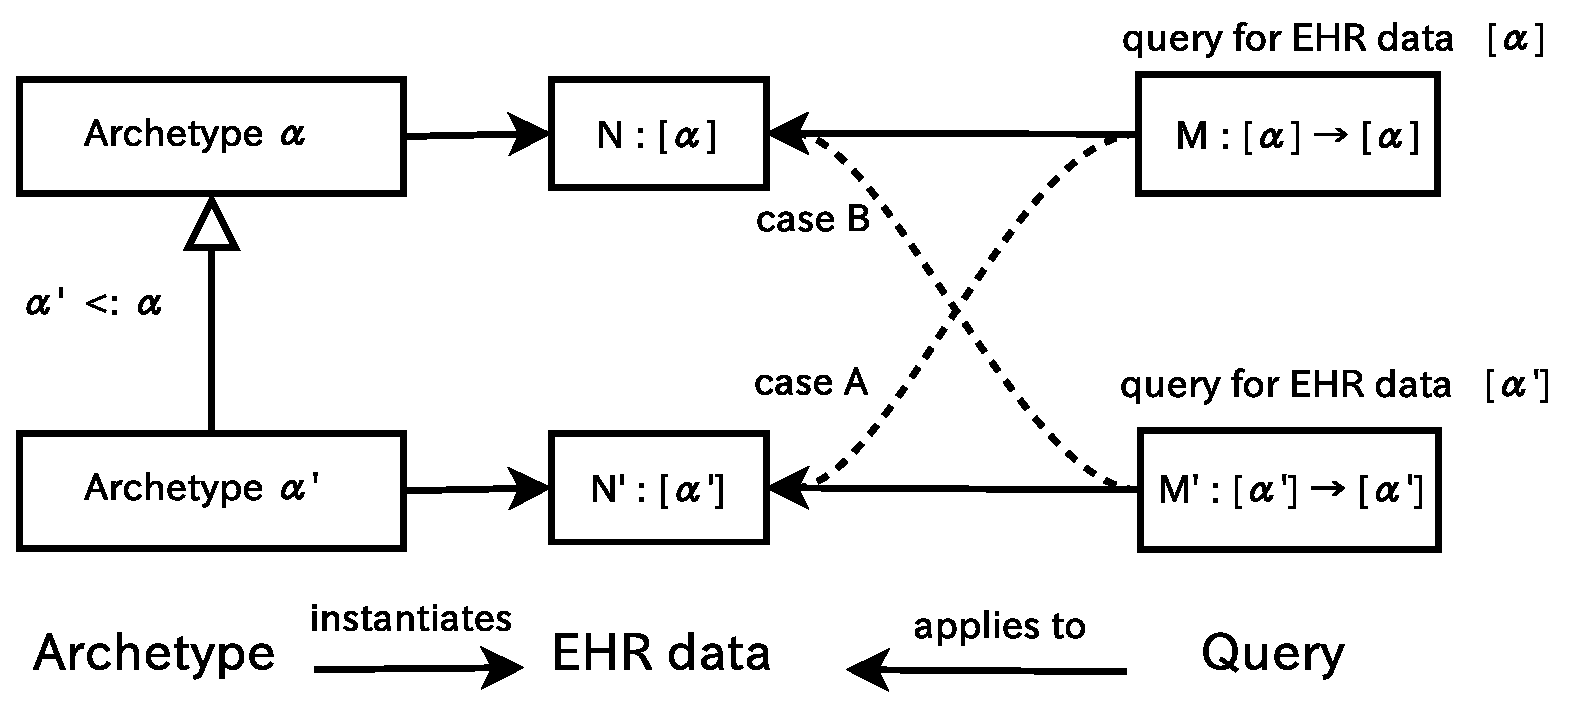
\includegraphics[width=10cm,clip]{archetype_based_queries.eps}  
  \end{center}
  \caption{Two cases of query applications}\label{fig:archetype_queries}
  This figure describes the relationships between archetypes, EHR data, and their queries. Four arrows are drawn from queries to EHR data. The two solid arrows indicate ordinary queries, the argument type of which is matched to the type of the EHR data (e.g., $M:[\alpha] \rightarrow [\alpha]$ and $N:[\alpha]$). The two dotted arrows indicate the cases for which we investigated the validity in the text. In case A, we are applying a query for a parent archetype $\alpha$ to the data created from its specialized archetype $\alpha'$. This is the case for {\bf Assertion 2}. In case B, in contrast, we are applying a query for a specialized archetype $\alpha'$ to the data created from its parent archetype $\alpha$.
\end{figure}


\begin{pf}
\begin{figure}[!htbp]
\begin{prooftree}
  \AxiomC{$\Gamma~ \vdash \alpha' <: \alpha$}
  \RightLabel{\quad [\ref{eqn:list_subtyping_rule}]}
  \UnaryInfC{$\Gamma~ \vdash [\alpha'] <: [\alpha]$}
  \AxiomC{$\Gamma~ \vdash N':[\alpha']$}
  \RightLabel{\quad [\ref{eqn:subsumption_rule}]}
  \BinaryInfC{$\Gamma~ \vdash N':[\alpha]$}
  \AxiomC{$\Gamma~ \vdash query~p:[\alpha] \rightarrow [\alpha]$}
  \RightLabel{\quad [\ref{eqn:application}]}
  \BinaryInfC{$\Gamma~ \vdash (query~p)~N':[\alpha]$}
\end{prooftree}\caption{Derivation of Assertion 2}\label{derivation_second_assertion}
Note that $\alpha$ is a parent archetype, $\alpha'$ is its specialized archetype, and $N' : [\alpha']$ is a list of EHR data created by the specialized archetype $\alpha'$.
\end{figure}
\end{pf}


The significance of this derivation is not so clear. Therefore, we presented the opposite case of applying a query for the specialized archetype $\alpha'$ to the data from the parent archetype $\alpha$. This assumption corresponds to case B in Fig. \ref{fig:archetype_queries}.
The query is encoded as $M' : [\alpha'] \rightarrow [\alpha']$, and the target database is encoded as $N:[\alpha]$. Then, it is obvious that $(M'~N)$ causes a type error, because $[\alpha']$ does not match $[\alpha]$ (cf., Eq.~\ref{eqn:application}). This indicates that queries based on a specialized archetype are not applicable to data created with the parent archetypes, whereas the queries based on the parent archetype can be reapplied to the data created by its specialized archetype.

\subsection{Archetypes should be invariant if they are mutable schema}

Section \ref{sec:howto_introduce_assignments} revealed that if we want to update EHR data, we must encode Archetype as $\mathsf{Archetype}\{l_i: \mathsf{Ref}(\tau^i) \}$ as in Eq.~\ref{eqn:mutable_record_field_reference}. Therefore, we need to determine how to derive the judgment $\mathsf{Archetype}\{l_1: \mathsf{Ref(\tau')} \}  <: \mathsf{Archetype}\{l_1: \mathsf{Ref(\tau)}\}$ based on the modified type system.

Subtyping of Reference types was defined in Eq.~\ref{eqn:reference_subtyping}.
We derived the tree shown in Fig. \ref{fig:derivation_mutable_archetype} by combining the mutable Archetype judgment and the Reference subtyping rules.

\begin{pf}
\begin{figure}[!htbp]
\begin{prooftree}
  \AxiomC{$\tau' <: \tau$}
  \AxiomC{$\tau <: \tau'$}
  \RightLabel{\quad [\ref{eqn:reference_subtyping}]}
  \BinaryInfC{$\mathsf{Ref(\tau')} <: \mathsf{Ref(\tau)}$}
  \RightLabel{\quad [\ref{eqn:archetype_subtyping}]}
  \UnaryInfC{$\mathsf{Archetype}\{l: \mathsf{Ref(\tau')} \}  <: \mathsf{Archetype}\{l: \mathsf{Ref(\tau)}\}$}
\end{prooftree}\caption{Derivation of the mutable archetype}\label{fig:derivation_mutable_archetype}
\end{figure}
\end{pf}

Figure \ref{fig:derivation_mutable_archetype} shows that subtyping of mutable archetypes depends on the type of $\tau$ and $\tau'$. However, $\tau' <: \tau \text{ and}~ \tau <: \tau' $ means that $\tau \text{ is equal to } \tau'$, because subtyping operator $<:$ is both transitive and reflexive (Eqs.~\ref{eqn:subtyping_reflexive} and \ref{eqn:subtyping_transitive}). Therefore, the derivation of Fig. \ref{fig:derivation_mutable_archetype} reveals that archetypes have to be invariant if they are mutable schemas.


Since this consequence is less intuitive, we demonstrate it through a counterexample. Based on Eq.~\ref{eqn:hypothesis}, let us assume that mutable archetypes are covariant. Based on this false hypothesis, we identify an inconsistency.

  \begin{alignat}{3}
  \text{Typing rules:} \qquad   \nonumber\\
    & \frac{\Gamma \vdash \tau'_i <: \tau_i  \qquad where~i \in 1..n+m}
           {\Gamma ~ \vdash \mathsf{Archetype}\{l_i: \mathsf{Ref(\tau'_i)} \}_{i \in 1..n+m}  <: \mathsf{Archetype}\{l_i: \mathsf{Ref(\tau_i)}\}_{i \in 1..n}} \label{eqn:hypothesis}
  \end{alignat}

Provided that type $\mathsf{Int}$ is integer and type $\mathsf{PosInt}$ is a positive integer, we assert that $\mathsf{PosInt} <: \mathsf{Int}$ by ad hoc rule, provided that $\mathsf{Archetype^A}\{l: \mathsf{Ref(PosInt)}\}$ and $\mathsf{Archetype^B}\{l_1: \mathsf{Ref(Int)}\}$. 

Then, since we assume the mutable Archetype to be covariant, $\mathsf{Archetype^A} <: \mathsf{Archetype^B}$. In addition, let us define $a \equiv archetype\{l = 1\} : \mathsf{Archetype^A}$ and $b \equiv archetype\{l = -1\} : \mathsf{Archetype^B}$. Given these settings, we can derive $a.l := -1$ as in Fig. \ref{fig:derivation_mutable_archetype_covariant}. This, however, contradicts $a.l : \mathsf{Ref(PosInt)}$, because $-1$ is {\it not} a positive integer.


\begin{pf}
\begin{figure}[!htbp]
\begin{prooftree}
  \AxiomC{$\mathsf{PosInt} <: \mathsf{Int}$}
  \RightLabel{\quad [\ref{eqn:hypothesis}]}
  \UnaryInfC{$\mathsf{Archetype^A} <: \mathsf{Archetype^B}$}
  \AxiomC{$a:\mathsf{Archetype^A}$}
  \RightLabel{\quad [\ref{eqn:subsumption_rule}]}
  \BinaryInfC{$a:\mathsf{Archetype^B}$}
  \RightLabel{\quad [\ref{eqn:record_projection}]}
  \UnaryInfC{$a.l:\mathsf{Ref(Int)}$}
  \AxiomC{$-1 : \mathsf{Int}$}
  \RightLabel{\quad [\ref{eqn:assignment}]}
  \BinaryInfC{$a.l := -1 : Unit$}
\end{prooftree}\caption{Derivation from the false hypothesis}\label{fig:derivation_mutable_archetype_covariant}
 Type $\mathsf{Int}$ is integer, and type $\mathsf{PosInt}$ is a positive integer.
\end{figure}
\end{pf}

As described above, if we allow EHR data to be updatable, then the semantics of the archetype is modified, and the variance of archetypes was changed from covariant to invariant.

\subsection{Archetypes should be both covariant and immutable}


Thus far, we have obtained different consequences of archetype variance from different premises. If the archetype is immutable, then the archetype is covariant, otherwise the archetype is invariant.
Both consequences are valid in terms of type theory.
As previously explained in Section \ref{sec:higher_concepts}, we need higher concepts than the type theory to decide which consequence is more appropriate. 
These higher concepts are 'structural interoperability' and 'schema extensibility'.


For the case in which the archetype is covariant, we can construct a specialized archetype along with its composition. As shown in Fig. \ref{fig:cohort_study}, when we specialize the {\sf RevisedCase} from the {\sf InitialCase}, we can also specialize its composition outcome from {\sf InitialOutcome} to {\sf RevisedOutcome}. For the case in which the archetype is invariant, we cannot specialize the components of the parent archetypes. Although this still guarantees structural interoperability, schema extensibility is still severely restricted. Comparing these two alternatives, we conclude that, for the sake of schema extensibility, the archetype should be immutable.


\subsection{EHR data are safe}


EHR data are created, validated, and queried based on their corresponding archetypes in ISO 13606. We defined the semantics in terms of the type system and clarified the behaviors of the semantics in terms of the derivations. However, we only inferred these derivations by symbolic manipulations referred to collectively as deduction and did not perform any evaluation such as queries or projections. Therefore, the simple question as to whether there are any discrepancies between the results obtained from the deductive proofs and the values of the EHR data from the actual evaluation results remains. The answer lies in the type theory.

A carefully constructed type system can take advantage of a property called {\bf soundness}.
If a type system is sound, then every derived judgment is assured to be valid, and the system is free from type errors \cite{mitchell00:_found_progr_languag,cardelli04:_type_system}.
This is the fundamental requirement of structural interoperability.
The soundness is stated in a more formal manner \cite[p.12]{cardelli04:_type_system} by Eq.~\ref{eq:soundness}, indicating that if M is an instance type $\tau$ (i.e., $M : \tau$), then M will be evaluated to obtain a value that has an inferred type of $\tau$.
Note that $\llbracket ~ \rrbracket$ is a function that evaluates a lambda term to obtain its value when applied to the term or infers the type of the term to obtain its simpler type when applied to the type itself.

\begin{equation}
  \label{eq:soundness}
  \text{if} ~~ \Gamma \vdash M : \tau ~~\text{is valid, then}~~ \llbracket M \rrbracket \in \llbracket \tau \rrbracket ~\text{holds.}
\end{equation}

Note that the aforementioned type system is sound \cite{gunter92:_seman_progr_languag,wright94:_syntac_approac_to_type_sound}, i.e., Eq.~\ref{eq:soundness} holds for every component of the proposed type system. We omit the soundness proof, because it is beyond the scope of this paper \footnote{Interested readers can refer to Fisher \cite{fisher94:_lambd_calcul_objec_method_special} or Wright \cite{wright94:_syntac_approac_to_type_sound} for a complete reference on the proof.}. Instead, we present an example in which the soundness holds.

Suppose term M is a projection function from $\mathsf{Archetype}\{l : \mathsf{TEXT}\}$ to $\mathsf{TEXT}$ (Eq.~\ref{eqn:example_evaluation_M_type}) and N is an instance of that archetype (Eq.~\ref{eqn:example_evaluation_N_type}). When we evaluate the term $(M~N)$, we obtain the value "text" from Eq.~\ref{eqn:evaluation_application}. On the other hand, when we infer the type of (M N), we obtain $\mathsf{TEXT}$ (Fig. \ref{fig:example_type_inference}).
Thus, $"text" \in \mathsf{TEXT}$ holds.

\begin{figure}[!htbp]
\begin{alignat}{3}
\text{provided that,} \quad  M & \equiv \lambda x:\mathsf{Archetype}\{l : \mathsf{TEXT}\}.(x.l) : \mathsf{Archetype}\{l : \mathsf{TEXT}\} \rightarrow \mathsf{TEXT} \label{eqn:example_evaluation_M_type}\\
                             N & \equiv archetype\{l = "text"\} : \mathsf{Archetype}\{l : \mathsf{TEXT}\} \label{eqn:example_evaluation_N_type}\\
\text{then,} \quad             \llbracket (M~N) \rrbracket & \Rightarrow_{\beta} "text" \label{eqn:evaluation_application}\\
                              & \text{where } \Rightarrow_{\beta}  \text{is called $\beta$-conversion that does } (\lambda x.M) N \Rightarrow_{\beta} M[x := N] \nonumber
\end{alignat}\caption{Evaluation of a lambda term $(M~N)$ }\label{fig:example_evaluation}
\end{figure}

\begin{pf}
\begin{figure}[!htbp]
\begin{prooftree}
  \AxiomC{$M : \mathsf{Archetype}\{l: \mathsf{TEXT}\} \rightarrow \mathsf{TEXT}$}
  \AxiomC{$N : \mathsf{Archetype}\{l : \mathsf{TEXT}\}$}
  \RightLabel{\quad [\ref{eqn:application}]}
  \BinaryInfC{$(M~N) : \mathsf{TEXT}$}
\end{prooftree}\caption{Type inference of a lambda term $(M~N)$}\label{fig:example_type_inference}
\end{figure}
\end{pf}

Although this is a small example, Eq.~\ref{eq:soundness} holds for every component, even for larger components such as EHR data, as long as the system is sound.
Then, we are justified in saying that the proposed sound type system guarantees the conformance of EHR data to their archetypes and that EHR data are safe in terms of type theory.

\section{Discussion}

In the present paper, we assigned major components of ISO 13606 to their proper types and derived multiple results for variance from different premises of mutability, using a deductive system of the type theory. As a result, we reached the conclusion that the archetype should be a covariant and immutable schema. Furthermore, we redefined the method of composing an archetype as uniquely designating the target archetype in an archetype slot.

In this section, we explain the importance of formal semantics, and discuss the assets and limitations of typed lambda calculus as compared with other formal methodologies that have been used in related research.
The novelty of our conclusion becomes clear when we present related research.


\subsection{Why formal semantics are needed}

The primary reason we could reach the above conclusion is that we built the formal semantics of ISO 13606. However, some readers might suspect that the primary subject of the standard is message modeling of EHR Extract, and such a conceptualized semantics is considered to be beyond the scope of the standard.
Indeed, the purpose of ISO 13606 is stated as follows:
\begin{quote}
  ISO 13606 may offer a practical and useful contribution to the design of EHR systems but will primarily be realized as a common set of external {\it interfaces} or {\it messages}.\cite[v]{iso08:13606_healt_elect_part1}
\end{quote}


However, semantics is an indispensable part of the standard and should be thoroughly investigated, even though the primary goal of ISO 13606 is in the specification of messages for communication of EHR data.

In informatics, the term message implies a grammatical arrangement of words rather than a substantial internal structure or behaviors. The validity of messages, however, depends on not only the grammar but also the semantics, an underlying principle for the internal structure and behavior. For example, "Plato loved Socrates" is a sensible sentence, whereas "Friday hates Saturday" is not, even though this sentence is grammatically correct. In other words, messages must conform to semantics, as well as to grammar. In these examples, the semantics is a constraint that restricts the domain of the function 'love' or 'hate' to human beings. The semantics underpins the validity of messages.

Semantics, despite its significance, is invisible, and thus appears unfamiliar. We can literally see the phrase "Plato loved Socrates" as an alphabetic sequence, but the function of 'love' itself, let alone its domain, is unclear. However, once we formalize the semantics, they can be visualized. When every term and rule is defined as a symbol, then inference can be seen as an arrangement of symbols, just as a sentence can seen as an arrangement of words. Then, we can easily explore the semantics. The inference mechanism rigorously excludes invalid results and derives novel results that we could never foresee. It is like the laws of physics, in terms of the degree to which they are conceptualized, which capture the true nature of the world as mathematical symbols and greatly expand the boundaries of our knowledge.


\subsection{Assets of typed lambda calculus}

We used typed lambda calculus as the formalization methodology, and there are several reasons why we chose this formalism.

First, typed lambda calculus has a long history of research in computer science as the computational model of statically typed programming languages. The theory laid the ground for not only typed functional languages, such as ML and Haskell, but also for object-oriented languages, such as Java \cite{igarashi01:_feath_java,barendregt13:_lambd_calcul_types}.
Second, type theory as a formalized deductive system is useful for proof-theoretic investigations \cite[p.9]{program13:_homot_type_theor}. We can construct proofs of already defined typed rules by properly combining the rules. Furthermore, the validity of the proofs depend only on the syntactic aspects thereof. This property of the theory helps us to check the proof, as we did in the present paper.
Third, the soundness of the type system ensures the validity of the consequences derived from the proof. If a value is proved to belong to a type, then the value must be exactly that type. This indicates that we can avoid erroneous operations of an EHR system that is built upon a sound archetype repository.

Typed lambda calculus guarantees a certain type of interoperability, referred to herein as structural interoperability, based on these properties. The knowledge and disciplines are so abstract and general that the results can be applied not only to ISO 13606, but also to every other standard in pursuit of the same goal.

\subsection{Related research}

We found two basic types of related research on formal semantics of archetypes. One type uses regular grammar theory \cite{jose09:_linkeh_ed,maldonado07:_framew_for_clinic_data_stand_based_archet}, and the other type uses Description Logic (DL) \cite{martinez-costa08:_model_driven_approac_for_repres,maldonado12:_using_resear_ehr,lezcano11:_integ_owl_swrl,martinez-costa10:_iso_en_openeh,costa12:_towar}.

Maldonado et al. \cite{jose09:_linkeh_ed,maldonado07:_framew_for_clinic_data_stand_based_archet} attempted to construct formal semantics of archetypes by means of regular grammar theory.  They abstracted archetypes as a tree with labeled nodes and developed a type system based on the concept of a constrained multiplicity list. They chose this approach because the functionality of archetypes resembles that of XML Schema, and the use of the regular grammar theory has been successful in building a formal theory of XML Schema \cite{chidlovskii00:_using_regul_tree_autom_xml,murata05:_taxon_of_xml_schem_languag}. These papers explained the semantics of archetype specialization and conformance of EHR data but did not investigate the issues of archetype variance or mutability as we did n the present study.

Several studies took a different approach, such as transferring archetypes to OWL, and these studies used DL, which is widely used as a theoretical foundation of ontology. Whereas most of these studies \cite{martinez-costa08:_model_driven_approac_for_repres,maldonado12:_using_resear_ehr,lezcano11:_integ_owl_swrl,martinez-costa10:_iso_en_openeh,costa12:_towar} simply translated archetypes to OWL without analyzing the semantics, Marcos et al. \cite{menarguez-tortosa13:_owl} attempted to analyze archetype semantics based on DL. They actually performed DL reasoning to check the consistency of archetypes and revealed that 22.2\% of the archetypes in the Clinical Knowledge Manager (CKM) repository and 21.2\% of the archetypes in the National Health Service (NHS) repository were inconsistent. However, their approach towards archetype consistency only considered archetype specialization, and they overlooked the problems of archetype variance and immutability, as in other previous studies.


Although type theory and logic are deeply related, as indicated by the Curry--Howard isomorphism \cite{lawler08:_class_logic_curry_howar_corres,sorensen98:_lectur_curry_howar_isomor}, type theory has several practical advantages over DL.
Since type theory is equipped with a deductive system, constructing proofs is easier than in DL, which has a set-theoretic background.
Furthermore, in typed lambda calculus, being a theoretical basis for modern programming languages, results are is easier to confirm or even implement compared to a DL-based approach.

\subsection{Limitations}

Typed lambda calculus has several advantages, and we have clarified some important aspects of archetype semantics that have been overlooked in previous studies. Despite these achievements, there are some limitations in this formalism. Specifically, whether type theory, which is inherently conservative due to its soundness, can cover the entire range of ISO 13606 archetype semantics remains unknown. Moreover, there are some difficult issues in encoding Archetype.

First, variant types prevent a schema from being extended, because its subtype has fewer choices than its supertype (Eq.\ref{eqn:variant_width_subtyping}). Suppose that we wanted to store a history of hepatitis and developed an archetype in which the choice of hepatitis is expressed as a variant type. Only hepatitis A and B were known to us at the time the archetype was developed, so we encoded the two alternatives as CODED\_TEXT.defining\_code (Fig. \ref{fig:example_variant_type}). Later, a problem was encountered when hepatitis C was discovered. Since the subtype of a variant type has fewer choices than the supertype (Eq.~\ref{eqn:variant_width_subtyping}), we cannot specialize the existing archetype. In order to avoid this inconvenience, we must define a new archetype that contains three types of hepatitis, namely, hepatitis A, B, and C. However, this approach is not extending the schema but only creating an additional schema, and this new schema is not able to reuse existing queries, as we showed in Fig. \ref{derivation_second_assertion}.

Second, it is difficult to encode an archetype model in which fields are parametrized by the RM type.
Even though we have shown how to express Archetype in typed lambda calculus, we intentionally ignored the fact that the field name of Archetype is partly dependent on the type of RM \cite[p.63]{iso08:13606_healt_elect_part2} and instead hard-coded the structure as a Record type.
For example, archetypes having an RM type of SECTION, such as CEN-EN13606-SECTION.substance\_use, should have a members field, whereas archetype having an RM type of ENTRY, such as CEN-EN13606-ENTRY.substance\_use, should have items and meaning fields. These fields cannot be parametrized according to the defined type system. Even if we try to introduce higher-order types \cite[p.24]{cardelli04:_type_system}, such attempts fail because the higher-order types parametrize only types and not the associated field names. We suspect that this type of parametrized archetype is very difficult to encode in any existing formalisms, including the regular grammar theory or DL.
  
\subsection{Prospectives}

As mentioned above, the proposed type theory did not cover the entire range of ISO 13606 archetype semantics.
This is partly because the theory may have some limitations, partly because ISO 13606 may go so far as to depart from the range of any formalisms, and partly because the type theory we introduced was too simple.
We believe that the coverage of the proposed theory can be widened if we add more type rules or extend the type system by adding more advanced features.

  First, bulk data structures, such as a list or a set, in ISO 13606 are parametrized according to the type of its elements, as in modern programming languages \cite[p.42]{iso08:13606_healt_elect_part1}.
These types can be correctly captured, if we introduce a recursive type to the proposed system \cite{cardelli04:_type_system,geuvers09:_introd_type_theor}.
  
Second, we did not discuss constraints on container attributes, such as cardinality, existence, occurrences, order, and unique \cite[p.83-84]{iso08:13606_healt_elect_part2}. The cardinality and occurrences constraints are difficult to handle because they are expressed as intervals, such as $\{0..1\}$ or $\{10..*\}$. The order and unique constraints, however, can be handled together so that we can determine a suitable type for each container. As the specification indicates \cite[xi]{iso08:13606_healt_elect_part2}, the proper collection type can be assigned according to the combination of order and unique constraints.

Third, ISO 13606 attempts to represent every conceivable type of health record data structure in a consistent manner \cite[vi]{iso08:13606_healt_elect_part1}, but the unit of measurement is one of the major exceptions. The units are expressed only as string representations, e.g., kg or mmHg \cite[p.46,p.82]{iso08:13606_healt_elect_part2}, not as a structured data type. This makes it difficult to properly convert or calculate EHR data according to their units. Type theory can address this problem when the units are constructed as a type \cite{kennedy94:_dimen_types,kennedy10:_types_units_measur}. Once we develop sound semantics, we can manipulate EHR data in a more consistent manner, such as automatic unit conversion or dimension-based validation.

These examples suggest that if we add more advanced features, we can enrich the semantics and extend the interoperability of ISO 13606 even beyond the reach of the original scope of the standard. In the future, we intend to encode and analyze the semantics of the ISO 13606 archetype with the latest results of the theory.


\section{Conclusions}

For ISO 13606, a solid foundation is necessary for the archetype semantics in order to achieve structural interoperability between EHR systems.
We analyzed the semantics by a formal methodology based on typed lambda calculus and clarified the following:

\begin{enumerate}
\item Archetypes should be both covariant and immutable schema, so that the structural interoperability is guaranteed and EHR schema are extended over time.
\item An archetype should uniquely specify other archetypes in the archetype slot when they are composed.
\end{enumerate}

We hope that the results of the present study would provide all who are involved in ISO 13606 a measure of insight and suggestions for the renewal tasks of the standard.

\section*{Acknowledgments}

The authors would like to thank Ms.~Mirai Ikebuchi for her advice on mathematical notations and for checking our derivations and Mr.~Yasuhide Miura for his assistance in preparing the manuscript.

The present study was supported in part by the Japan Society for the Promotion of Science (JSPS) through the Funding Program for World Leading Innovative R\&D on Science and Technology (FIRST program).

\bibliographystyle{elsarticle-num-names}
%\bibliographystyle{apalike}
%\bibliographystyle{elsarticle-num}
%\bibliographystyle{abbrvnat}
%\bibliographystyle{unsrtnat}
%\bibliographystyle{plainnat}
%\bibliographystyle{plain}
%\bibliographystyle{IEEEtran}
%\bibliographystyle{nci}
%\bibliographystyle{vancouver}
\bibliography{books}

\end{document}

%%% Local Variables: 
%%% mode: japanese-latex
%%% TeX-master: t
%%% End: 






